\chapter{Multi-objective Evolution based Dynamic Job Scheduler in Grid}

\section{Problem Definition}
Grid is a distributed decentralized heterogeneous computational system, later it has also incorporated network storage system. User applications run on Grid varies from lightweight to extensive computational/storage application with various constraints. Job Scheduler is responsible to select best suitable machines in this grid for each job. In large grid this should be done automatically. The scheduling system generates job schedules for each machine in the grid by considering predefined static constraints of jobs and machines and dynamic behavior of grid. Grid environment is highly dynamic, resources can join and leave grid any time.\\
We define the problem in three sections as follows: 
\subsection{Flexible Job Shop Scheduling}
The typical job-shop problem is formulated as a work order that consists of set of $n$ jobs, each of which contains $m$ tasks. Each task has predecessors and requires a certain type of resource, i.e. to be processed by any machine from a given set \cite{wall1996genetic}. Often many resources of a specific type are available, for example five milling machines and two lathes. Many tasks can be assigned to any one of the available resources, but the resource must be of the suitable type. Similarly in the computing environment some computational jobs have certain requirement specifications and resource types to maintain their quality of service. Typical objectives for scheduling include minimizing the makespan for the work order. Here we are also considering energy consumption, time limit constraint, cost constraint and maximize utilization of resources as objectives.
\subsection{Dynamic Scheduler}
Dynamic scheduler considers dynamic environment of grid where resources can change its configuration and availability. In dynamic scheduling re-evaluation is allowed for already taken assignment decisions during job execution \cite{chtepen}. It can trigger job migration or interruption based on dynamic information about the status of the system and the workload. When a resource leaves grid system the Grid Information Service (GIS) can trigger the scheduler to reschedule the queued jobs among the available resources. However care should be taken on scheduling the jobs that are dependent on the rescheduled jobs. Similarly addition of new resources will trigger reshuffling of the jobs for proper utilization of resources though less complexities are involved in this case. Section ~\ref{dynamicscheduling} addresses this problem.
\subsection{Gridlet}
Grid job is often referred to as Gridlet. Jobs can be fine as well as coarse grained. In grid computing, MI is the unit of job size. MI is million instructions or processing requirements of a user job \cite{liao2009research}. If the MI of a job is less than a fixed threshold $M$, it is a fine-grained job. Similar approach i.e. Megabytes(MB) parameter is used for storage intensive jobs. For fine-grained jobs, a job-grouping strategy is suggested for faster execution of scheduler in section ~\ref{jobgr}.
\begin{figure}[ht]
    \centering
    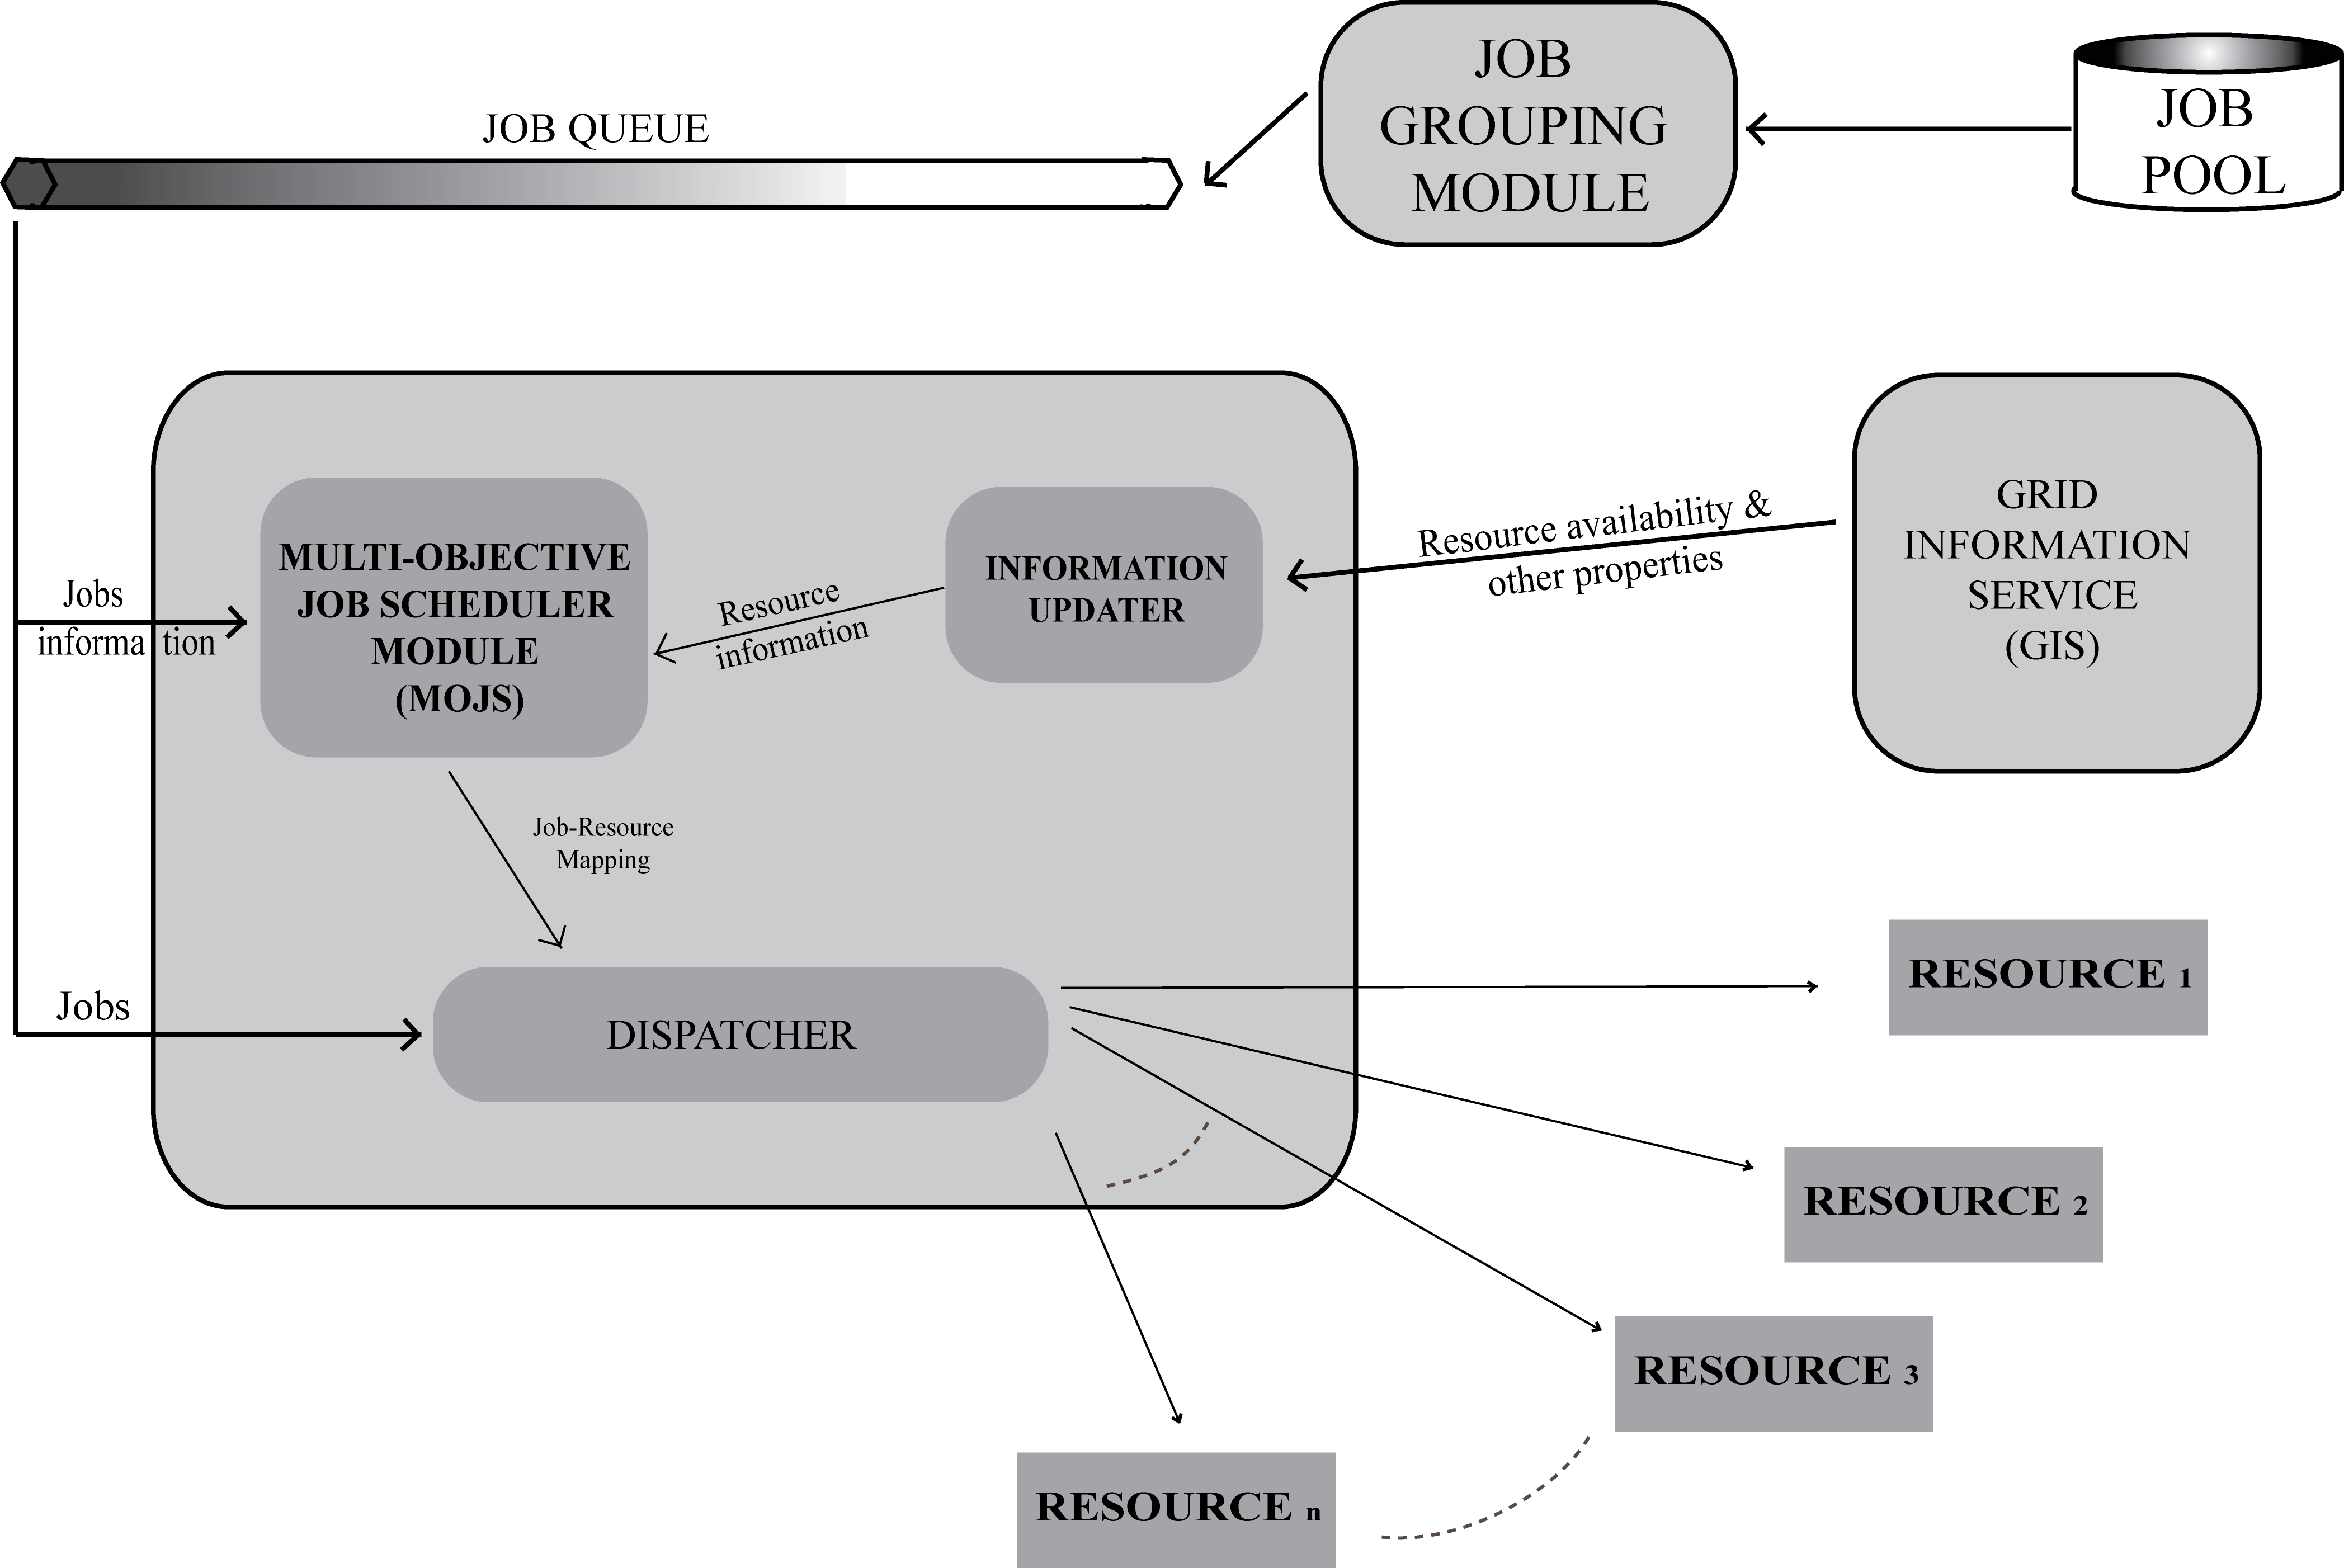
\includegraphics[width=1.0\columnwidth]{scheduler}
    \caption{Scheduling Model}
	\label{fig:Scheduling Model}
\end{figure}

\section{Job Scheduling Model}
The four basic building blocks of grid model are as follows 
\begin{itemize} 
 \item Users 
 \item Job scheduler 
 \item Grid Information System (GIS) 
 \item Resources
\end{itemize}
 The user submits a list of jobs to the job pool where it gets a unique identification number i.e. Job ID. If necessary job-grouping of very fine-grained jobs is accomplished by meta-scheduler before the scheduler process these jobs. The scheduler obtains information of resources from Grid Information Service (GIS). GIS provides information like resource availability, processing capability, energy consumption and cost details. Based on the information, a scheduling strategy i.e. mapping of jobs with execution start time and resources is created and send to dispatcher. The dispatcher dispatch jobs to their corresponding resources on time and collects the results of completed jobs from the resources.

\section{Formulation of problem}
\label{formulation}
Here the problem is formulated with the notations described in scheduling literature \cite{brucker2004scheduling}, \cite{brucker2006scheduling}, \cite{jakob2008fast}. Given are a set $M = \{M_1, M_2, M_3, ... M_m\}$ of resources, a set $J = \{J_1, J_2, J_3, ... J_j\}$ of application jobs, and a set $O$ of grid jobs. The n Grid Jobs of application job $J_i$ are denoted by $O_{i1},..., O_{in}$, a set $W= \{W_1,W_2,\ldots,W_m\}$ denotes normalized energy dissipation factor of resources. Table ~\ref{notation1} gives a concise definition of the notations have been used.\\
\begin{table}[!ht]
\caption{Notation Symbol and their definitions}
\centering
    \begin{tabular}{|c|l|}
    \hline \hline
    Notation & Definition  \\ \hline
    $M_i$ & Resource with ID $i$ \\ \hline
    $J_i$ & Application job with ID $i$ \\ \hline
    $O_{ij}$ & $j$th Grid Job or task of Application job $J_i$ \\ \hline
    $W_i$ & Energy dissipation factor of Resource $M_i$, \\
	  & normalized with the max value from set $W$ \\ \hline
    $t(O_{ij},R_{ij})$ & Processing time of $O_{ij}$ mapped to resource $R_{ij}$ \\ \hline
    $c(O_{ij},R_{ij})$ & Cost of $O_{ij}$ mapped to resource $R_{ij}$ \\ \hline
    $s(O_{ij})$ & Start time of job $O_{ij}$ \\ \hline
    $e(O_{ij})$ & End time of job $O_{ij}$ \\ \hline
    $d_{ij}$ & Time limit for completion of $O_{ij}$ \\ \hline
    $c'_{ij}$ & cost limit for  $O_{ij}$ \\ \hline
    $tsum(M_i)$ & Running time or Uptime of $M_i$ \\ \hline
    \end{tabular}
\label{notation1}
\end{table}
\textbf{The following functions are used:}
\begin{itemize}
  \item A precedence function 
  \subitem $p:O$x$O \rightarrow \{ TRUE,FALSE\}$ for the grid jobs.
  \item An assignment function $\mu:O \rightarrow P(P(M))$ from grid jobs to resource sets. $P(M)$ is the power set of $M$. $\mu_{ij}$ is the set  of all possible combinations of resources from $M$, which together are able to perform the grid job $O_{ij}$
  \item Resource mapping $R: O \rightarrow P(P(M)) $, $R_{ij}$ represent mapping of job $O_{ij}$ on a machine $M$, $R_{ij} \in \mu_{ij}$
  \item Function $t:O$x$P(M) \rightarrow \mathbb{R}$, which gives for every grid job $O_{ij}$ the time needed for processing on a resource set $R_{ij} \in \mu_{ij}$
  \item Cost function $c: O$x$P(M) \rightarrow \mathbb{R}$, $c(O_{ij},R_{ij})$ is the cost of job $O_{ij}$ mapped on resource $R_{ij}$.
  \item Function $l:M_i  \rightarrow O_{jk}$ which gives the last grid job executed on resource $M_i$
  \item Function $s:O_{ij} \rightarrow \mathbb{R}$, $s(O_{ij})$ is the start time of grid job $O_{ij}$.
  \item Function $e:O_{ij} \rightarrow \mathbb{R}$, $e(O_{ij}) = s(O_{ij}) + t(O_{ij},R_{ij})$ is the end time of grid job $O_{ij}$ which is mapped on resource $R_{ij}$.
  \item Function $tsum : M_i \rightarrow \mathbb{R}$ which gives the resource $M_i$ running time or Uptime.
\end{itemize}
Optimization is done by choosing suitable start times $s(O_{ij}) \in \mathbb{R}$ and resource allocations $R_{ij} \in \mu_{ij}$. A solution is valid, if the following two \textbf{restrictions} are met:
\begin{enumerate}
  \item All grid jobs are planned and resources are allocated exclusively:
  \subitem $ \forall O_{ij} : \exists s(O_{ij}) \in \mathbb{R}, R_{ij} \in \mu_{ij} : \forall M_j \in R_{ij} $:
  \subitem $M_j$ is in $[s(O_{ij});s(O{ij})+t(O_{ij}),R_{ij}]$ exclusively allocated by $O_{ij}$
  \item Precedence relations are adhered to: 
  \subitem $\forall i, j \neq k : p(O_{ij},O_{ik}) \Rightarrow s(O_{ik}) \geq s(O_{ij}) +t(O_{ij}, R_{ij})$
\end{enumerate}
Exceeding the time limit and budget cost will affect QoS of grid jobs. A penalty factor is imposed when jobs violates following \textbf{constraints}.
\begin{enumerate}
  \item All grid jobs $O_{ij}$ have time limit $d_{ij}$ which must be adhered to:
  \subitem $ \forall O_{ij} : d_{ij} \geq s(O_{ij}) + t(O_{ij},R_{ij}) $:
  \item All grid jobs $O_{ij}$ have a cost limit  $c'_{ij}$ which must be adhered to: 
  \subitem $\forall O_{ij} : c'_{ij} \geq c(O_{ij},R_{ij}) $
  
\end{enumerate}
\textbf{This work focuses on achieving near-optimal scheduling strategy on following objective functions}:
\begin{enumerate}
  \item Minimizing makespan, $e(O_{ij})$ is the end time of grid job $O_{ij}$
  \subitem $ f_1 =makespan = max\{e(l(M_1)),e(l(M_2)),\ldots,e(l(M_m)) \}$
\begin{framed}
Makespan is the time at which all the resources becomes free.
\end{framed}
  \item Maximizing utilization of resources i.e. minimizing $f_2$
  \subitem $ f_2 = non-utilization = \frac{1}{m} \sum_{j=1}^{m}  \{e(l(M_j)) - tsum (M_j)\}$
\begin{framed}
$f_2$ is the average time period during which the the resources are idle.
\end{framed}
  \item Minimizing time limit penalty (minimizing number of jobs completing after due date)

$$
f_3 = \frac{1}{j*n}  \sum_{\forall i,j} \varphi _1 (e(O_{ij}) - d_{ij}) 
$$
where $\varphi _1(x)$ is a non-negative continuous exponential non-decreasing function, if $x > 0$ else $0$.

\begin{framed}
The grid jobs failed to complete within time limit contribute to the \par penalty function $f_3$. Minimizing time limit penalty is our aim.
\end{framed}
  \item Minimizing cost penalty 
$$
f_4 = \frac{1}{j*n}  \sum_{\forall i,j} \varphi _2 \{c(O_{ij},R_{ij}) - c'_{ij}\} 
$$
where $\varphi _2(x)$ is a non-negative continuous linear non-decreasing function, if $x > 0$ else $0$.

\begin{framed}
The grid jobs failed to meet the cost limit constraint contribute to the \par penalty function $f_4$. Minimizing cost limit penalty is our aim.
\end{framed}
  \item Minimizing Overall Energy consumption
  \subitem $f_5 = \sum_{i=1}^{m} tsum(M_i) * W_i$
\begin{framed}
$f_5$ gives energy consumption of all the resources.
\end{framed}
\end{enumerate}

\section{MOJS Module}
On submission of jobs and grid resource infromation to Multi-Objective Job Scheduler (MOJS) module, it outputs a near optimal scheduling strategy. Some of the important building blocks of scheduler are discussed below.
\subsection{Multi-objective optimization}
Generalized multi-objective optimization problem can be described as:\\
Minimize $y = f(x) = (f_1(x),f_2(x),\ldots,f_k(x))$\\
where $x \in \mathbb{V}, y \in \mathbb{R}^k$\\
where, $x$ is decision vector in search space $\mathbb{V}$, $y$ is the objective vector with $k > 1$ objectives.
\subsection{Chromosome model}
A scheduling strategy or mapping of jobs on resources satisfying the constraints is represented by  chromosome. A chromosome stores parameters as follows 
\begin {itemize}
\item Resource id corresponding to each job
\item Start time of every job
\item End time of every job
\item Predecessor job ID of each job 
\item Five objective function values 
\item Rank of chromosome, Rank is defined in section ~\ref{nds} 
\item Crowding distance, defined in section ~\ref{cds} 
\end{itemize}
Start time for execution of jobs is calculated according to heuristic rules (i) Schedule grid job as early as its precedent job is completed (ii) Schedule grid jobs according to shortest due date.
\subsection{Non-Dominated Sorting}
\label{nds}
A chromosome $a$ is said to be dominated by chromosome $b$ iff $\forall i \in \{1,2,\ldots,k\}: f_i(a) \leq f_i(b)$ and $\exists i \in \{1,2,\ldots,k\}: f_i(a) < f_i(b)$.
A chromosome $a$ is said to be Non-dominated if there does not exist any chromosome $b\in \mathbb{V}$ search space that dominates $a$. A set of such non-dominated chromosome in objective space is called pareto optimal front. After removing the pareto optimal front, a second pareto optimal front can be obtained. We assign a rank to each of the chromosome according to their occurrence in the pareto front. Then the algorithm sorts the population according to their rank and crowding distance (discussed in section~\ref{cds}) for selecting population for next generation. After a certain number of generations any chromosome from the first pareto front satisfying the soft constraints  can be chosen as the near optimal solution, or a weighted sum of the objectives can be used for finding suitable solution.
\subsection{Diversity preservation}
It is desired that the evolutionary algorithm maintains a good spread of solutions in the population, so that sustainable diversity in the population remains and solutions are not restricted to local optimization.
\subsubsection{Crowding distance}
\label{cds}
Crowding distance ($dist_x$) of a particular chromosome $x$ in population measures the density of chromosomes surrounding it. \\
After non-dominated sorting is completed, each chromosome's crowding distance is calculated as the sum of normalized distance between its adjacent neighbors corresponding to each objective. Crowding distance for first and last individual is infinite.\\

$dist_x = \sum _{j=1}^{k}\frac{f_j(x_{left})-f_j(x_{right})}{f_j^{max} -f_j^{min}}$
where $f_j$ is $j$th objective function, and number of objectives is $k$.
\subsubsection{Crowded comparison operator}
Each chromosome in the population will have two attributes
\begin{enumerate}
\item non-domination rank $r_x$
\item crowding distance $dist_x$
\end{enumerate}
\begin{framed}
A partial order $\prec$ between chromosomes are defined as:\\
$ a \prec b $ if $r_a \prec r_b$\\
or $(r_a = r_b)$ and $(dist_a \succ dist_b)$
\end{framed}
This means that we prefer a chromosome from less crowded region in search space in same front.
\subsection{NSGA II}
Non-dominated Sorting Genetic Algorithm II \cite{deb2002fast} is used as a basic framework for our Job scheduler module. In NSGA II, initially a random parent population $P_0$ is created. Using the above relation partial order population is sorted. For the first generation binary tournament selection, recombination, and mutation operators are used to create an offspring population $Q_0$ of same size as $P_0$ say $N$.\\
Now we describe the $t$th generation. A combined population $R_t = P_t \cup Q_t$ is formed of size $2N$. Then $R_t$ is sorted according to non-domination. Now best non-dominated set i.e. first pareto front $F_1$ is chosen for new population. If size of $F_1$ is less than $N$ then solutions from $F_2$ are chosen next, followed by $F_3$ and so on. Now a new population $P_{t+1}$ of size N is chosen  after crowding distance sorting.  This population is now used for selection, crossover, mutation to generate new offspring population $Q_{t+1}$ of size $N$ , and $R_{t+1}$ is formed by union of $P_{t+1}$ and $Q_{t+1}$. A schematic explanation of procedure is given in Figure ~\ref{NSGA2}.
\begin{figure}[!h]
    \centering
    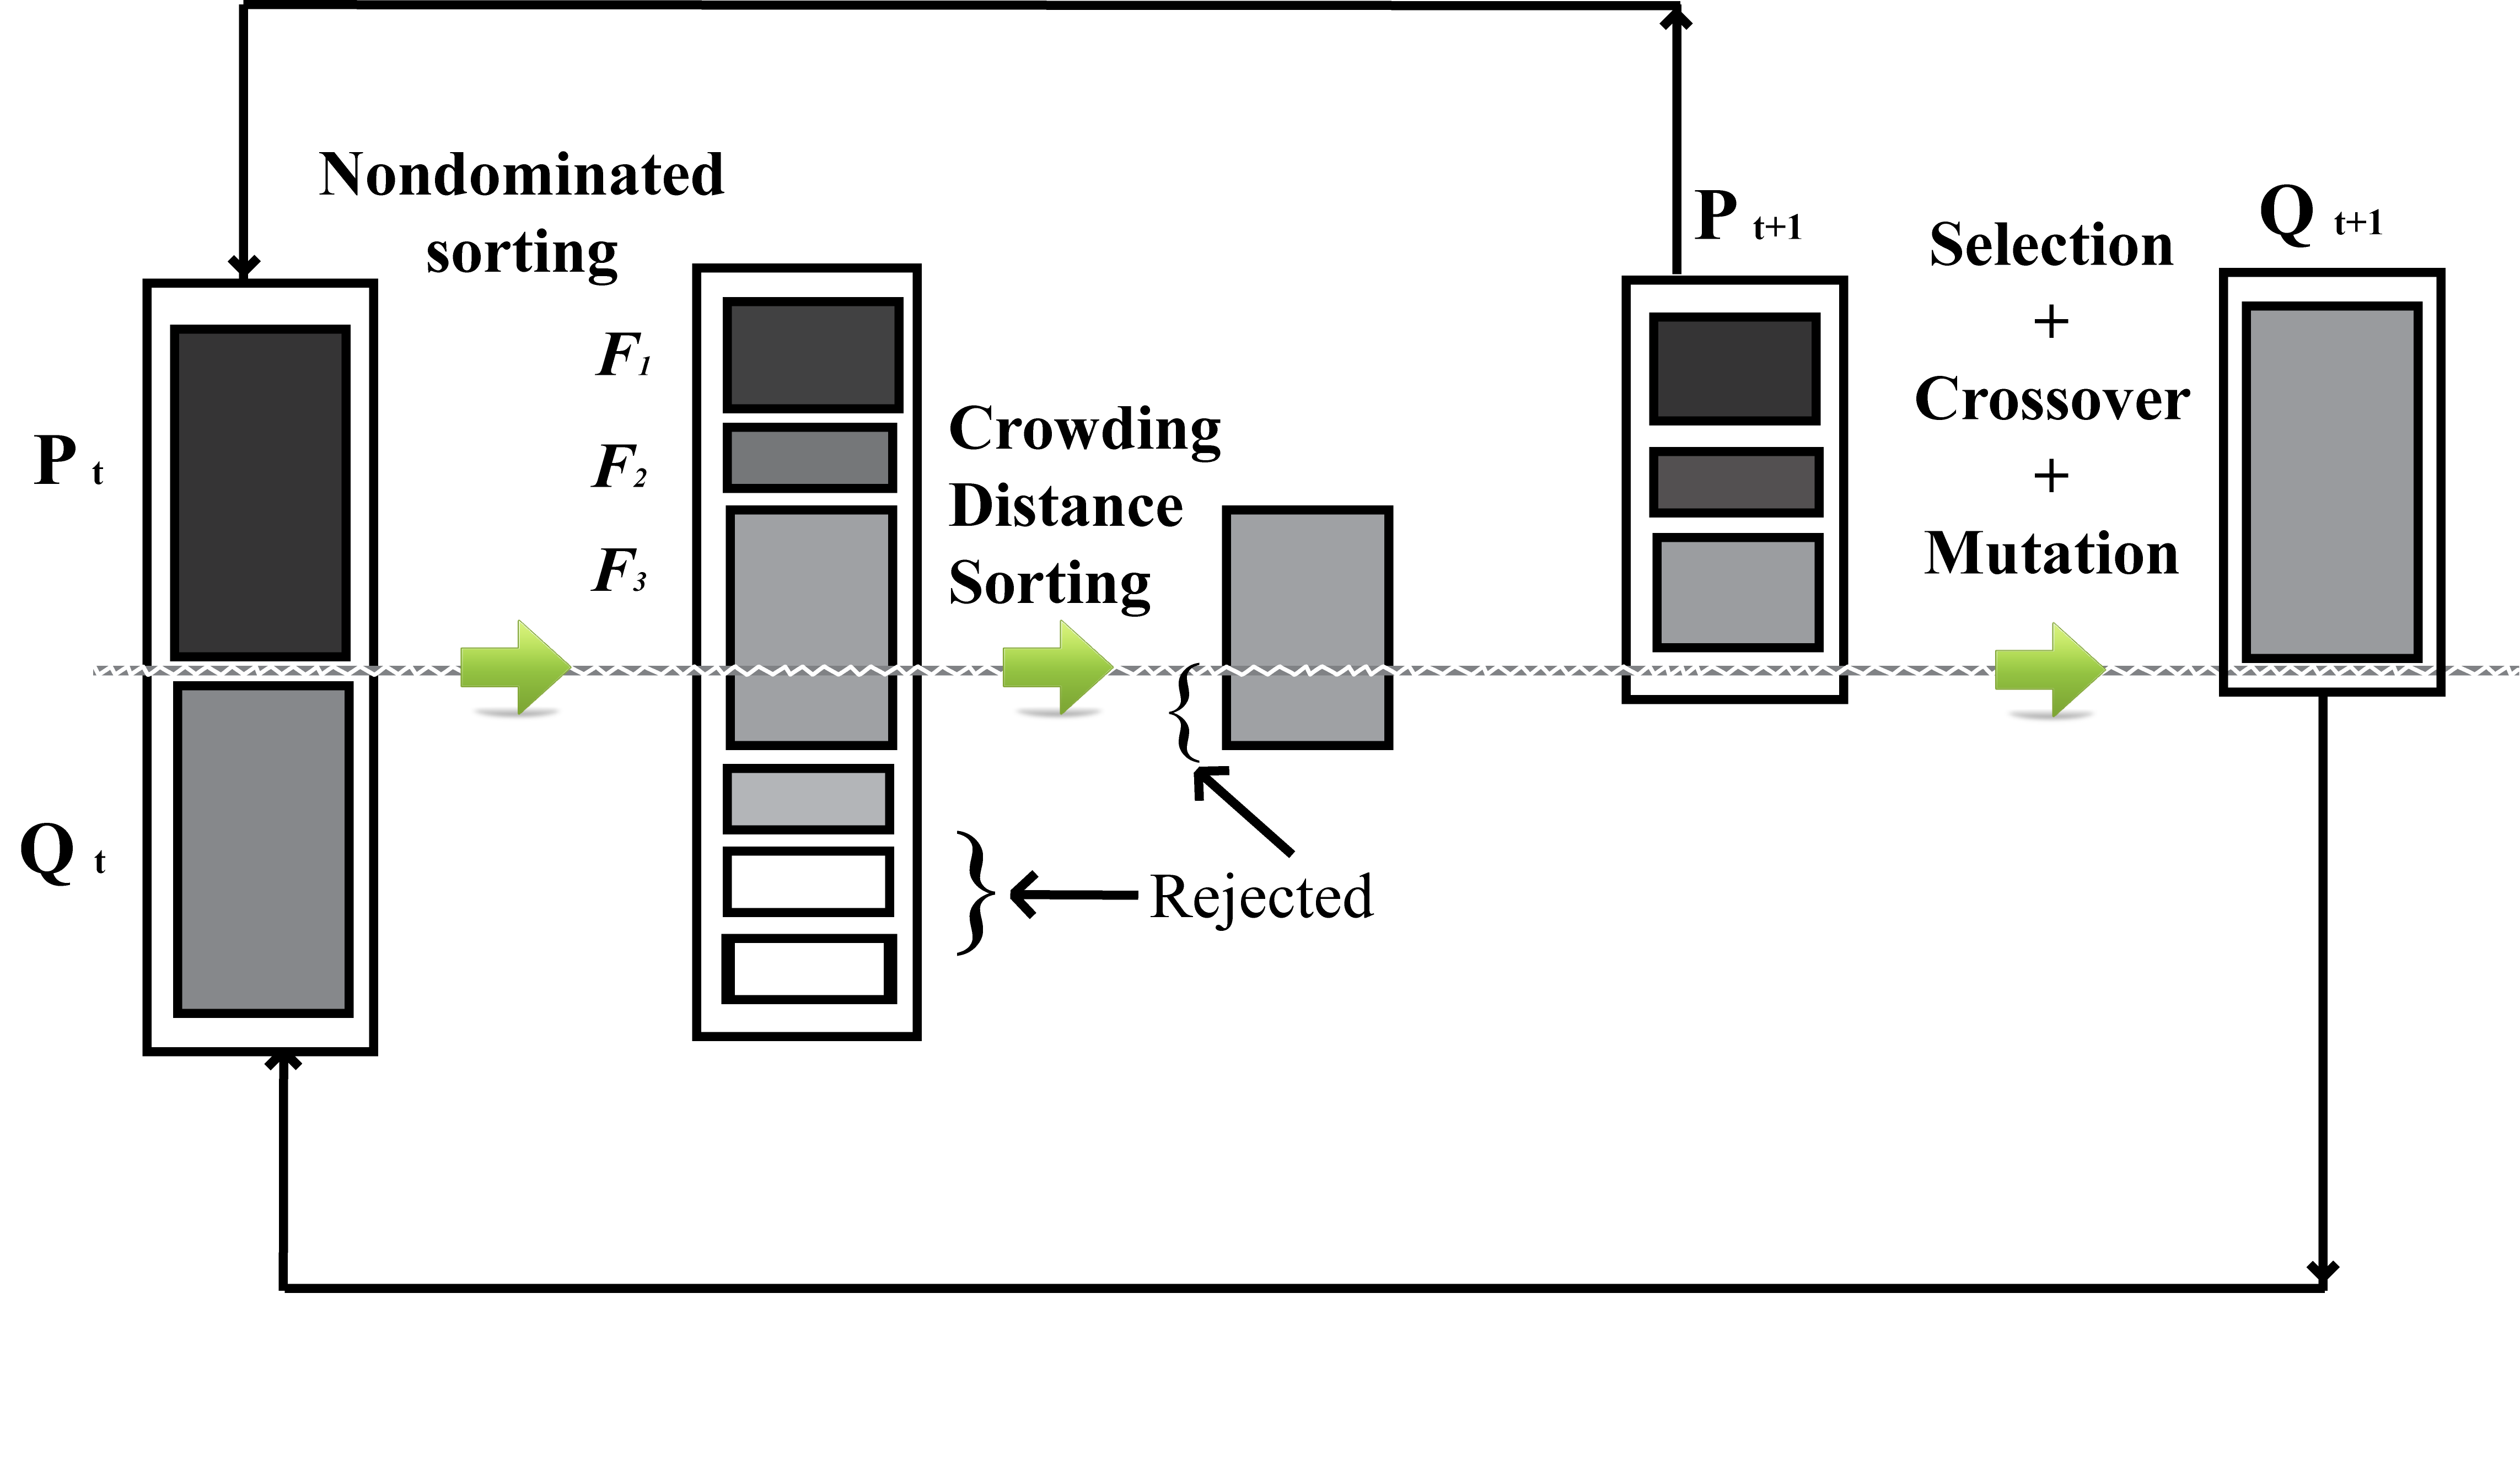
\includegraphics[width=1.0\columnwidth]{NSGA2}
    \caption{NSGA II procedure \cite{deb2002fast}}
	\label{NSGA2}
\end{figure}
\subsection{Crossover, Mutation and Elitism}
\subsubsection{Crossover}
The crossover operators are the most important part of any evolutionary-like algorithm. In each generation a mating pool of chromosomes is created through a tournament of selection among chromosomes. Two chromosomes are selected from mating pool interchanging their genes to obtain new individuals. The aim is to obtain new individual/chromosome with better fitness function and that will help in exploring new regions in search space not explored yet. $P_c$ is the probability with which crossover operator is applied.
Crossover operators depends on the chromosome representation.\\
\textbf{\emph{One point crossover: }} Given two parent chromosomes, this operator first randomly chooses a position between 1 and $NUM\_JOBS$. The point act as cutting point. Then the two first parts of the parents are interchanged yielding two new descendants. Schematic representation is given in Figure ~\ref{1pointxover}.\\
\begin{figure}[!h]
    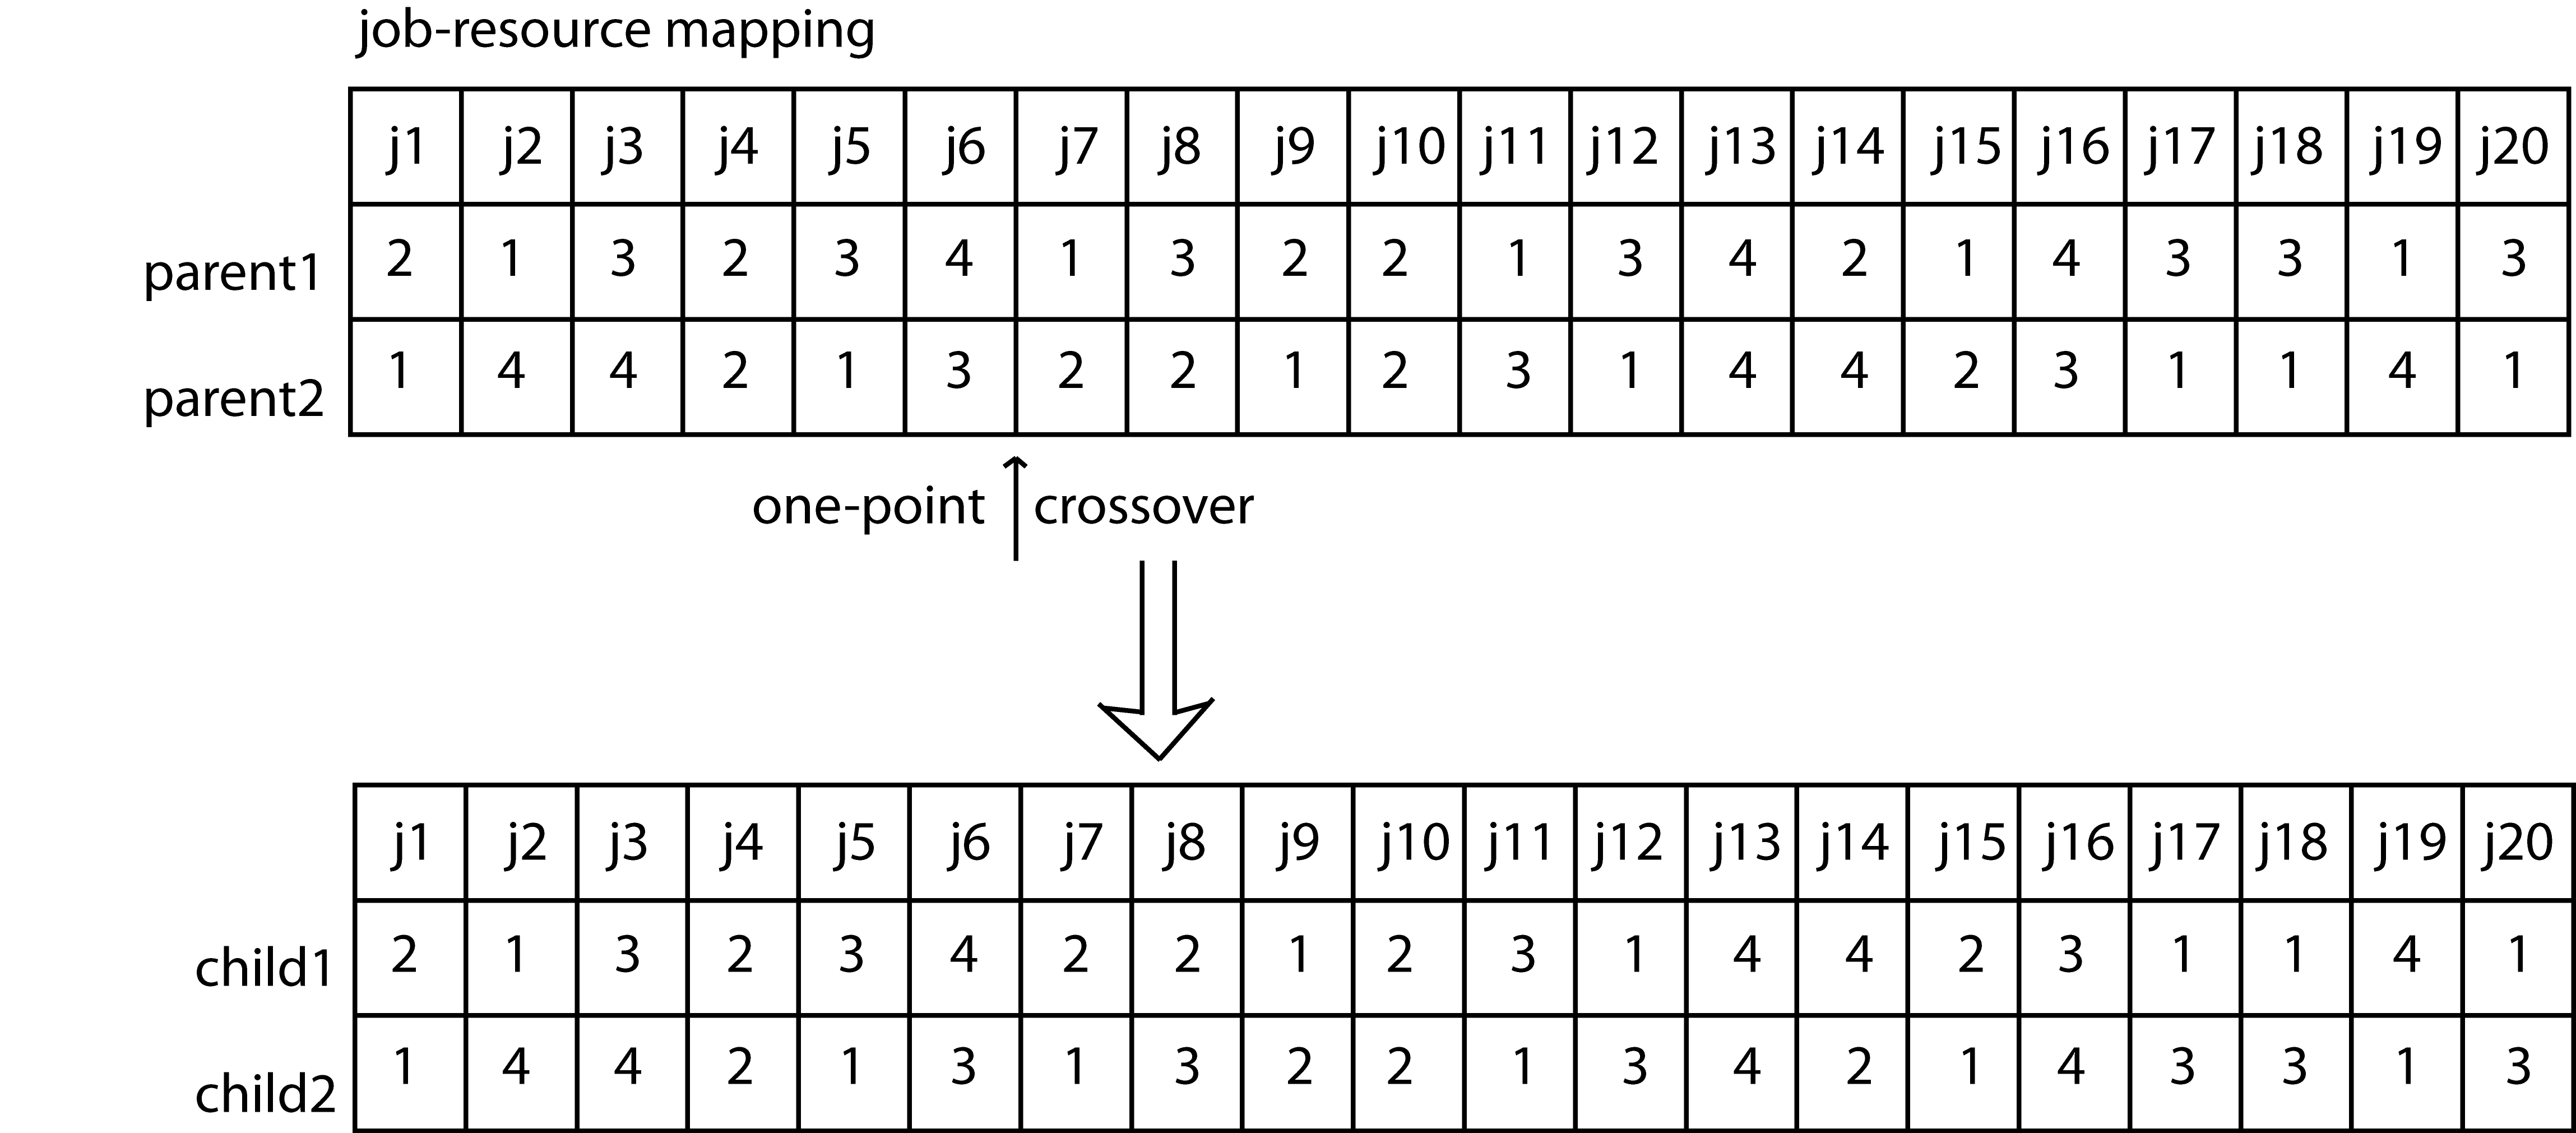
\includegraphics[width=1.0\columnwidth]{crossover1}
    \caption{One point crossover}
	\label{1pointxover}
\end{figure}
\begin{figure}[!h]
    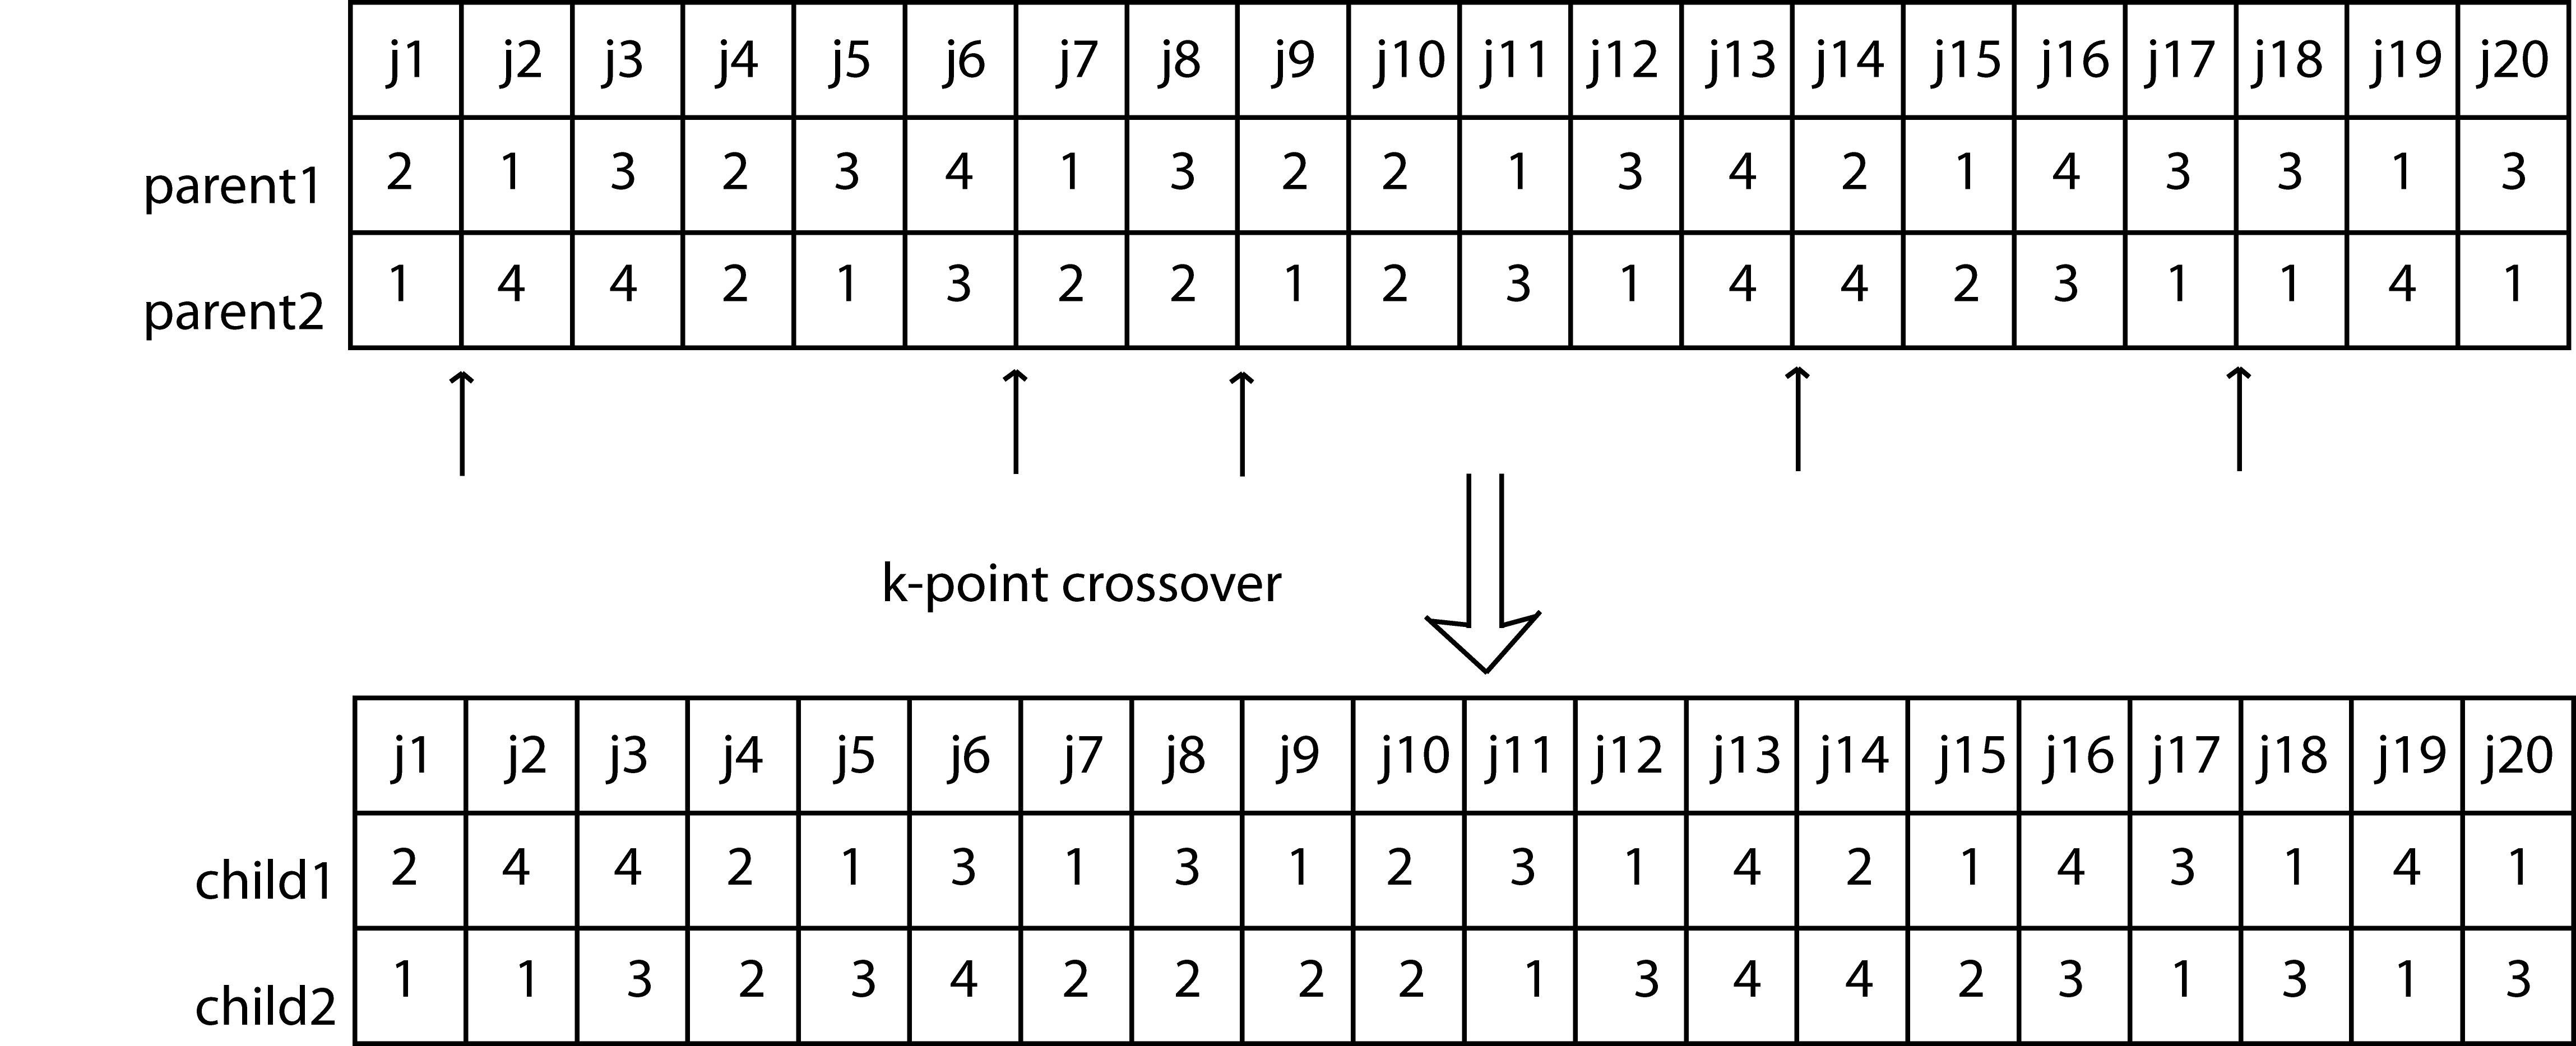
\includegraphics[width=1.0\columnwidth]{crossover2}
    \caption{k-point crossover}
	\label{kpointxover}
\end{figure}
\textbf{\emph{k-point crossover: }} This operator is a generalization of one-point crossover. Two or more cutting points i.e. $k \geq 2$ are randomly chosen and segments are interchanged alternately yielding two new descendants. However it should be noticed that large value of $k$ tends to explore more thoroughly the solution space but it is likely that it will destroy parents structure. An example is given in Figure ~\ref{kpointxover}.\\
\textbf{\emph{ Mask Crossover: }} A mask array of 0/1's is created randomly of size $NUM\_JOBS$ i.e. $mask = m_1,m_2,m_3,\ldots,m_{NUM\_JOBS}$ where $m_i = 0/1$. Figure ~\ref{mcrossover} explains this operator.
$$
\forall i, chromosome_{new_1}[i] = \left\{ \begin{array}{rl}
 chromosome_{parent_1}[i] &\mbox{ if $m_i = 0$} \\
 chromosome_{parent_2}[i] &\mbox{ otherwise}
       \end{array} \right.
$$
$$
\forall i, chromosome_{new_2}[i] = \left\{ \begin{array}{rl}
 chromosome_{parent_1}[i] &\mbox{ if $m_i = 1$} \\
 chromosome_{parent_2}[i] &\mbox{ otherwise}
       \end{array} \right.
$$
\begin{figure}[h]
    \centering
    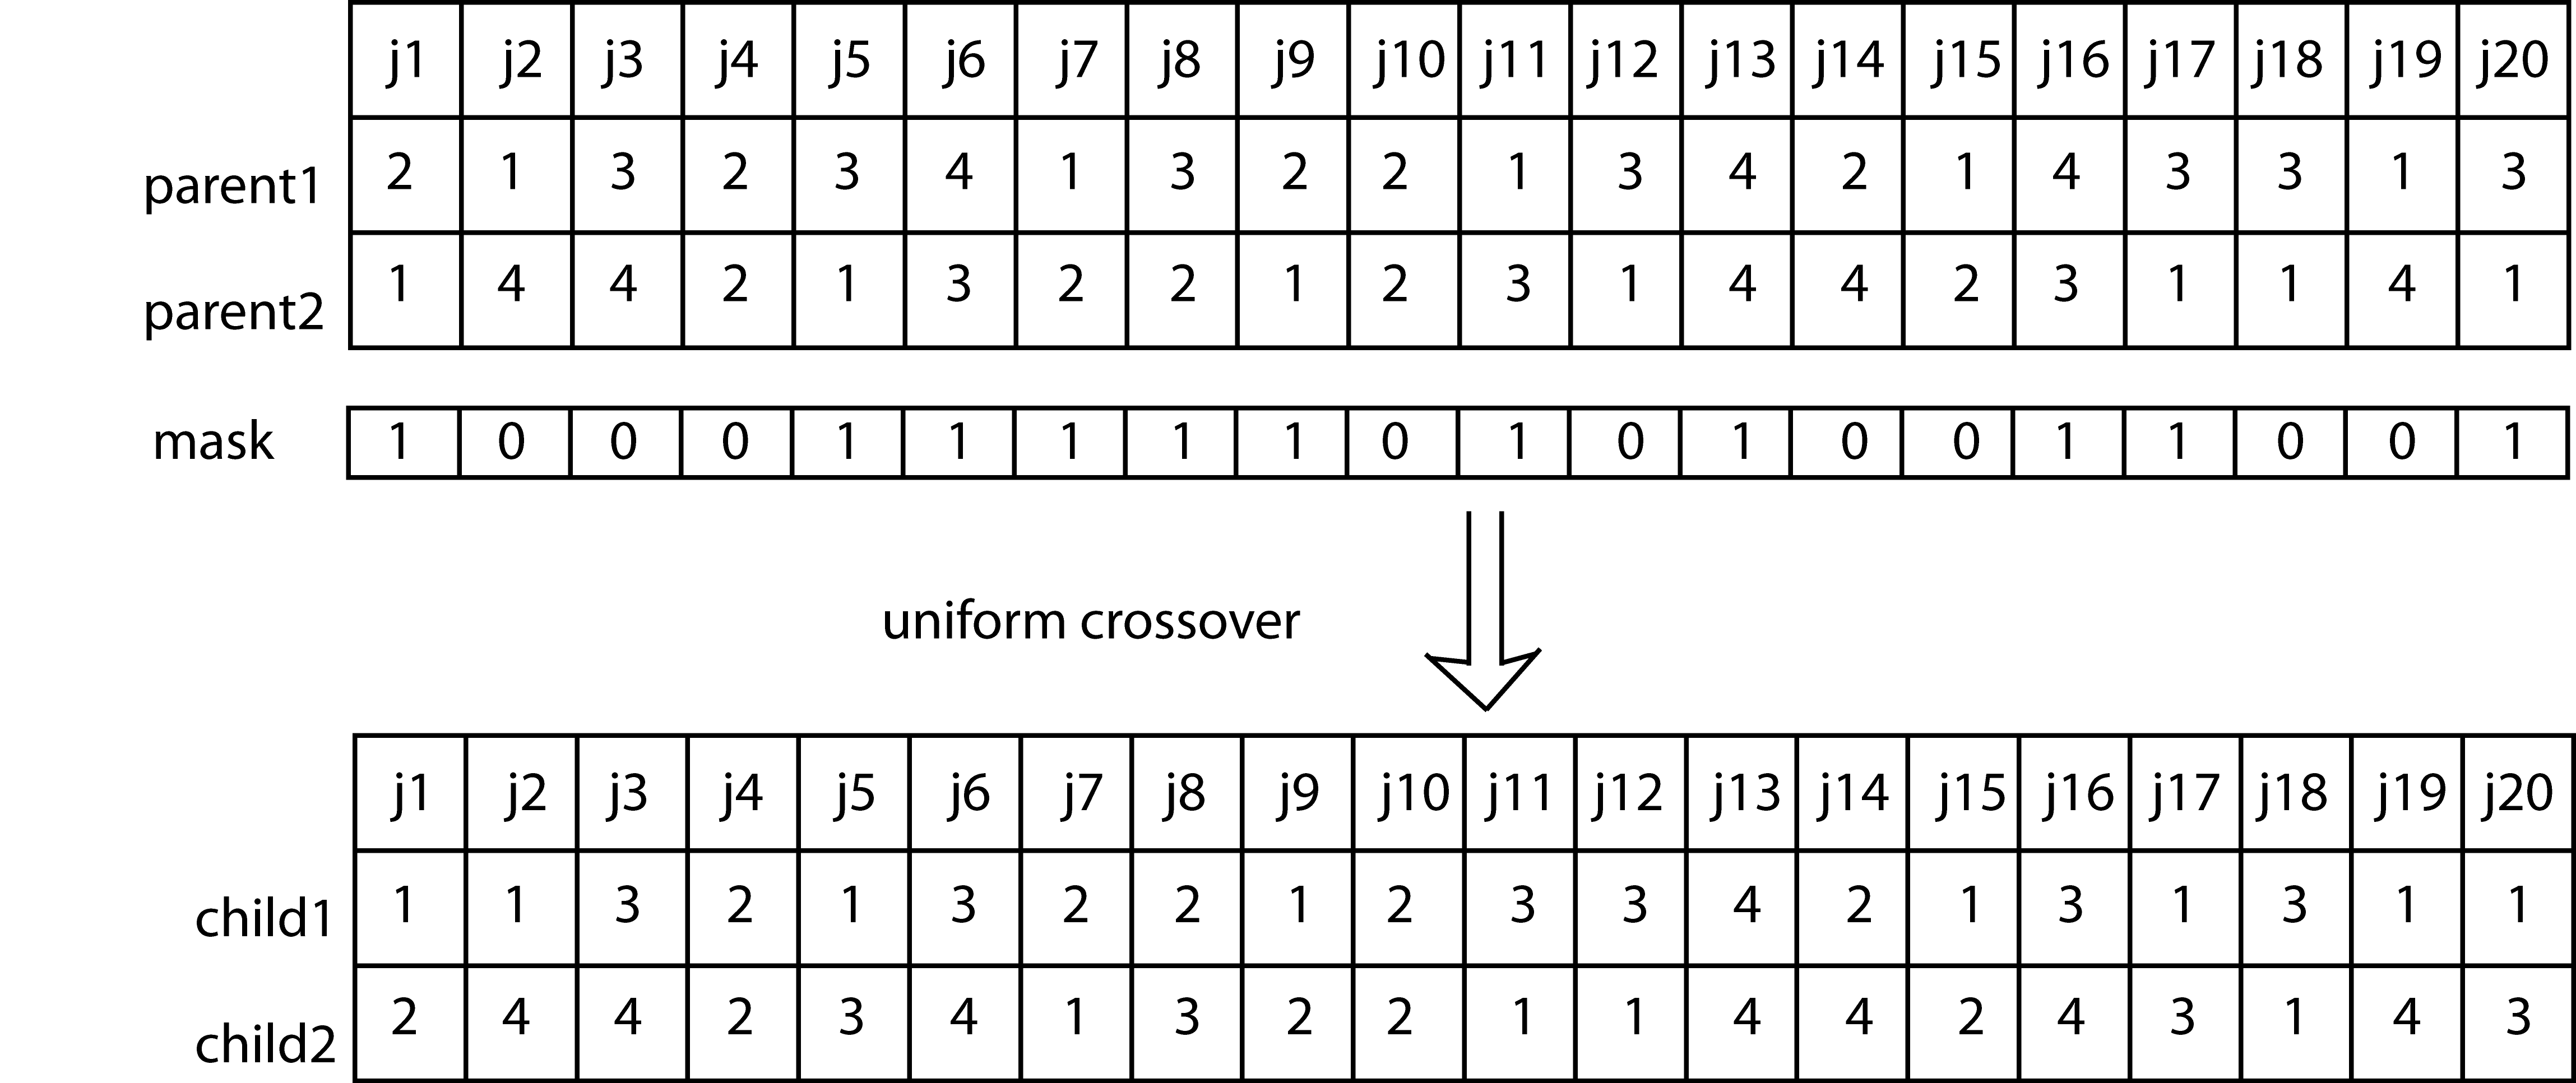
\includegraphics[width=1.0\columnwidth]{crossover3}
    \caption{Mask crossover}
	\label{mcrossover}
\end{figure}
\textbf{\emph{Fitness based Crossover: }} In this operator fitness or any other external function can be used. Our approach yield two descendants. The crossover is computed as follows. Working methodolgy can be inferred from Figure ~\ref{fitcrossover}.\\
$$
\forall i, chromosome_{new_1}[i] = \left\{ \begin{array}{rl}
 chromosome_{parent_1}[i] &\mbox{with probability $p = \frac{g_1[i]}{g_1[i] +g_2[i]}$} \\
 chromosome_{parent_2}[i] &\mbox{with probability $1-p$}
       \end{array} \right.
$$
$$
\forall i, chromosome_{new_2}[i] = \left\{ \begin{array}{rl}
 chromosome_{parent_1}[i] &\mbox{with probability $p = \frac{h_1[i]}{h_1[i] +h_2[i]}$} \\
 chromosome_{parent_2}[i] &\mbox{with probability $1-p$}
       \end{array} \right.
$$
\begin{figure}[t]
    \centering
    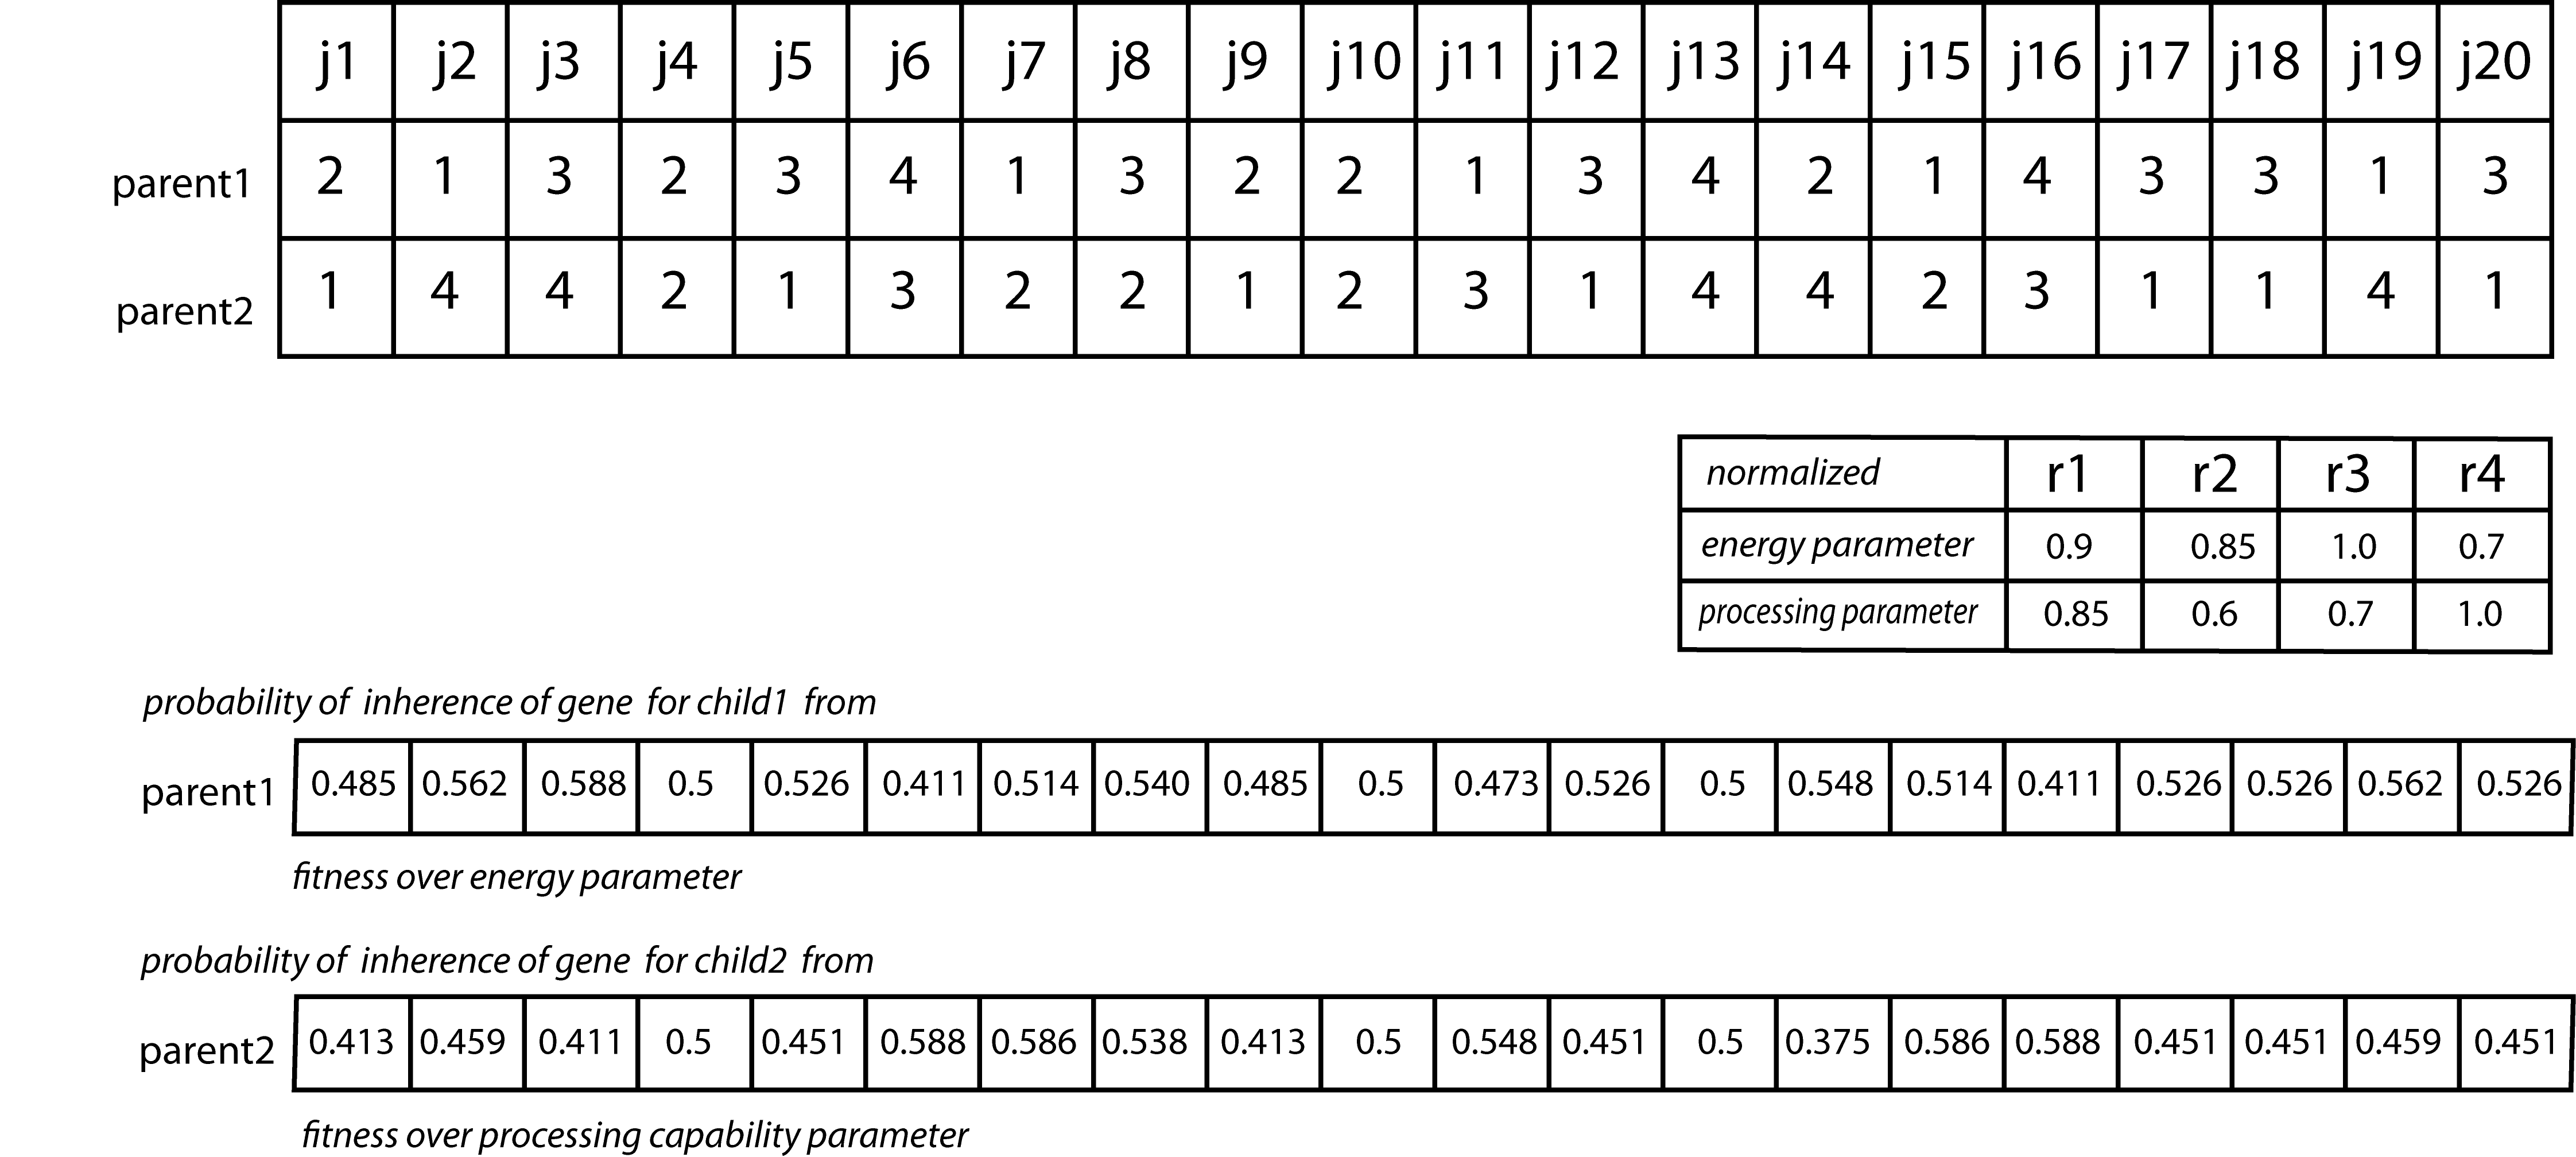
\includegraphics[width=1.0\columnwidth]{crossover5}
    \caption{Fitness based crossover}
	\label{fitcrossover}
\end{figure}
Each resource in grid has processing capability and energy efficiency parameter. They almost counteract each other and need a tradeoff between them to find optimal schedule.\\
Here  $g_1[i], g_2[i]$ are energy efficiency parameter of $chromosome_{parent_1}[i]$ and $chromosome_{parent_2}[i]$ respectively.
Similarly $h_1[i], h_2[i]$ are processing capability parameter of $chromosome_{parent_1}[i]$ and $chromosome_{parent_2}[i]$ respectively.
\subsubsection{Mutation}
$P_m$ is the probability with which mutation operator is applied. Mutation operators used as follows.\\
\textbf{\emph{ Move:}} This operator randomly assigns a resource to the job. Care is taken that resource type is same i.e. resource belongs to same set.\\
\textbf{\emph{ Swap:}} This operator randomly chooses two jobs and swap their assigned resources if they belong to same set.\\
\textbf{\emph{ Rebalancing: }} This operator takes into account number of jobs assigned to each resource. This operator chooses most overloaded resource and randomly pick a job assigned to it. Then the job is moved to a resource which is less overloaded.\\
\begin{figure}[ht]
    \centering
    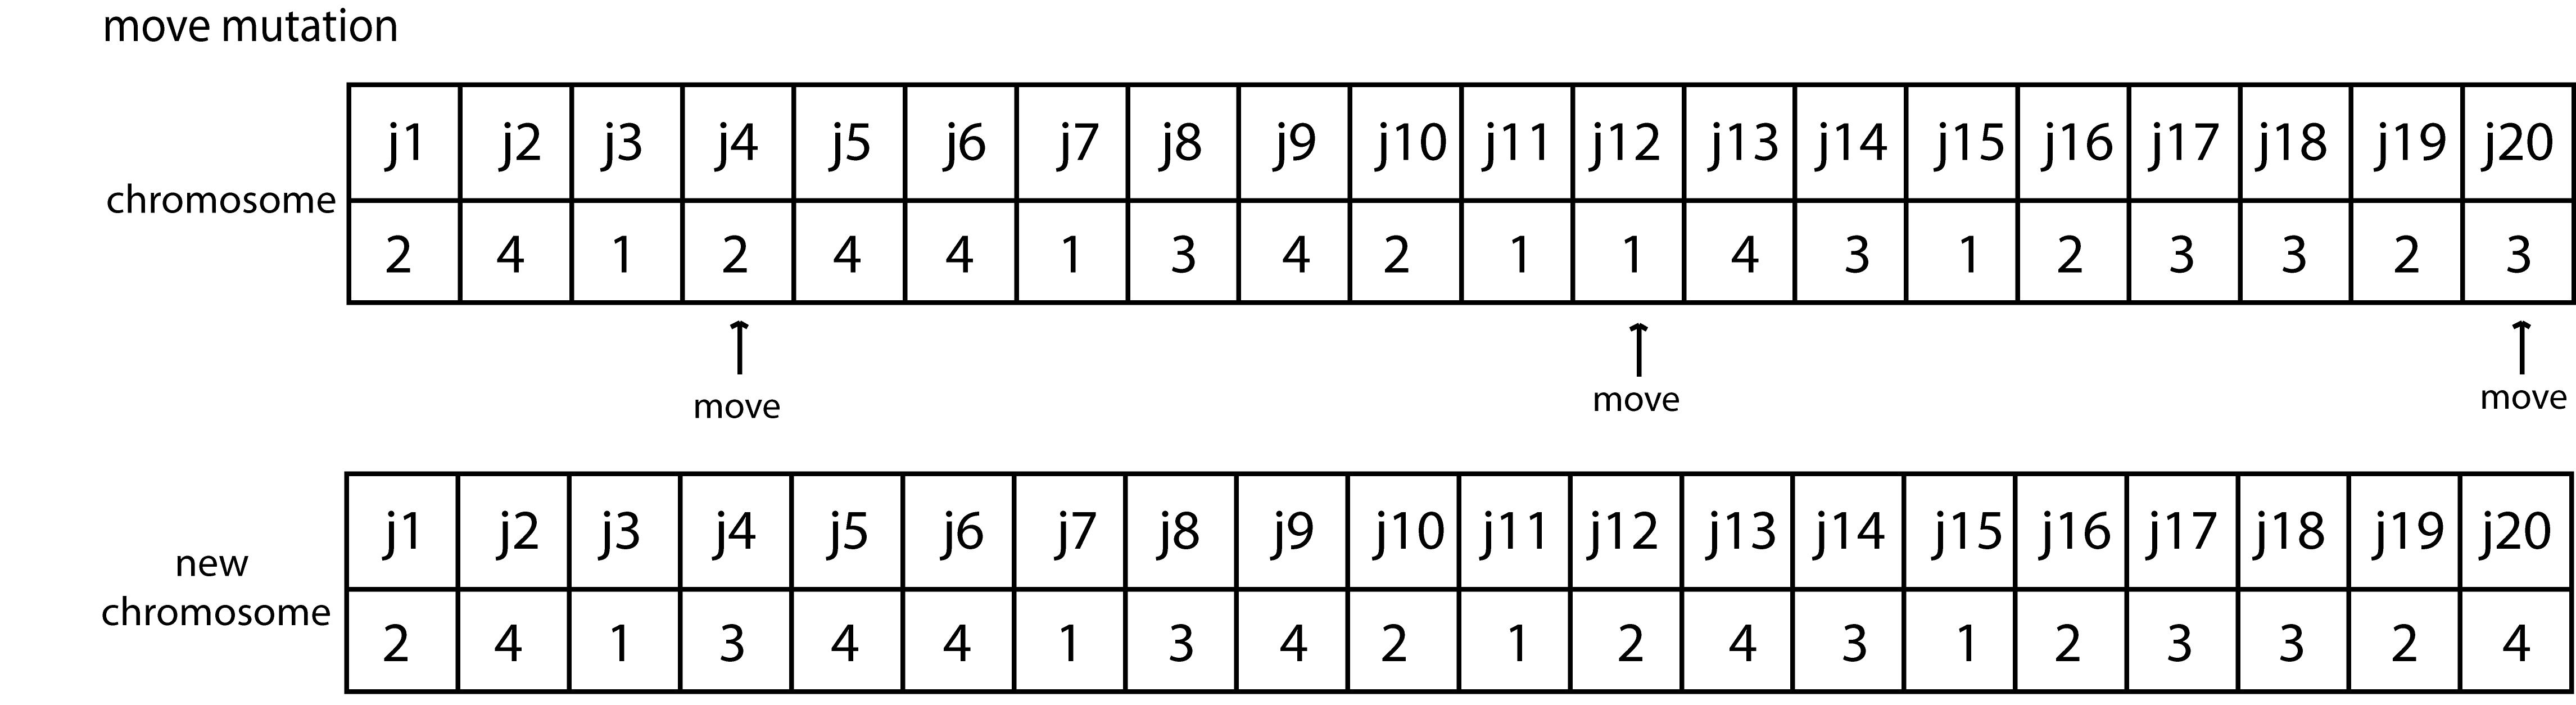
\includegraphics[width=1.0\columnwidth]{mutation1}
    \caption{Mutation- move}
	\label{movemuta}
\end{figure}
\begin{figure}[h]
    \centering
    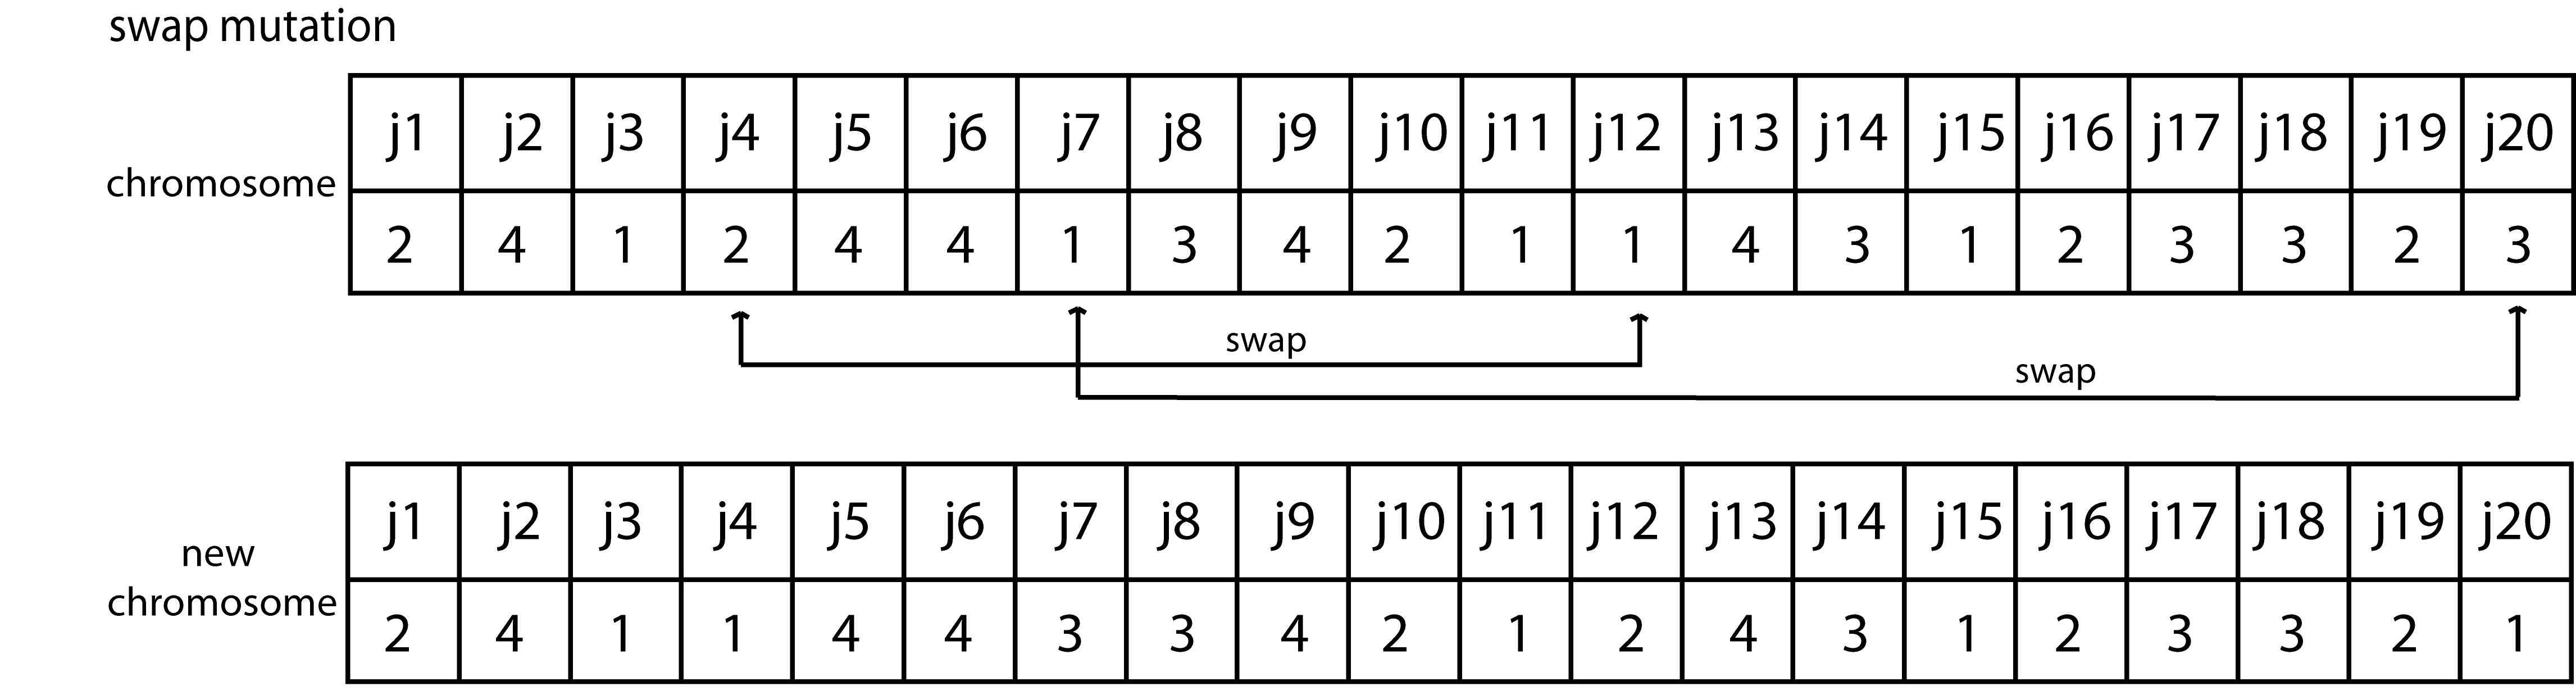
\includegraphics[width=1.0\columnwidth]{mutation2}
    \caption{Mutation- swap}
	\label{swapmuta}
\end{figure}
\subsubsection{Elitism}
In the process of crossover and mutation it is possible that some good chromosomes might be lost. Elitism is a mechanism to preserve these chromosomes. A small percentage of the fittest population i.e. first pareto front in multi-objective search space is forwarded to be the part of new population for next iteration.
\section{Dynamic scheduling}
\label{dynamicscheduling}
Application jobs queued in grid are fed to the MOJS module in batch. The output is the elitist pareto front of chromosomes comprises near optimal schedules. Soft constraints and weighted sum approach is applied on multiple objectives to finalize a chromosome as scheduling strategy. Some jobs are queued on their respective resource while others are again fed to MOJS module. The number of jobs queued depend on the fitness of the chromosome and time available for the scheduler to re-run and find a better schedule. Progress is ensured by setting a minimum number of jobs to be queued on a single run of module. \\
As this is a real time scheduling problem and resources are dynamic in nature it can participate and leave the system any time, it is of higher importance to make the scheduling dynamic in nature. By dynamic we mean re-allocation of already scheduled jobs which were not completed. So change in the resource pool can trigger running of scheduler which can either reschedule the jobs whose resources have left the grid or can request processing of new jobs on addition of one or more resources or both of them. Jobs whose predecessors is present in the set of rescheduled jobs are also rescheduled. \\
There is very little scope for this paper to solve the issue where a job suffers starvation and penalty due to failure of resource. To handle this issue accounting of Mean Time to Failure (MTTF) with log mining can help.
\section{Job Grouping for Fine-grained Jobs}
\label{jobgr}
Fine grained jobs are grouped to form a single job. Following are the constraints considered while job grouping.
\begin{itemize}
 \item Jobs grouped as single job should be of same type i.e. either computational jobs or storage intensive jobs. 
 \item Prevail same job precedence rule after job grouping.
\end{itemize}
Workflow and precedence of jobs is represented through Directed Acyclic Graph (DAG), where nodes are jobs and directed edge represents precedence. \\
A directed edge from $a$ to $b$ is drawn, when $b$ awaits for the completion of job $a$ and $a$ is said to be the predecessor of $b$ and $b$ is the successor of $a$. Nodes having common edge are defined as adjacent nodes. We define $a,b$ to have same job type if their resource type requirement is same.\\
Before we present our heuristic algorithm for job-grouping, we define few terms as follows:
\subsection{Entry job}
A job without any predecessor but has atleast one successor is called entry job. If there are multiple entry jobs for a DAG component then we add a zero size job/node and new directed edges are drawn from zero size job to entry jobs. Hence we have a single entry job denoted as $j_{entry}$.
\subsection{Exit job}
A job without any successor but has atleast one predecessor is called exit job. If there are multiple exit jobs for a DAG component then we add a zero size job/node and new directed edges are drawn from  exit jobs to zero size job. Hence we have a single exit job denoted as $j_{exit}$.
\subsection{Job size}
Size of a computational job is measured in Million Instructions(MI) and storage jobs in Megabytes(MB). It is denoted as $job\_size(j)_{computational}$ or $job\_size(j)_{storage}$. 

\begin{framed}
{\small
\emph{Note:}
\begin{itemize}
\item A computational job has $job\_size(j)_{storage} =0$ MB
\item A storage job has $job\_size(j)_{computational}=0$ MI
\end{itemize}
}
\end{framed}

\begin{algorithm}[ht]
\caption{job grouping}
\begin{algorithmic}
\REQUIRE { Job pool with DAG representation }
\STATE {Compute $crit_{up}(j)_{<type>}$ for each job $j$   according to the equation ~\ref{eq:up1} }
\STATE {Compute $crit_{down}(j)_{<type>}$ for each job $j$ according to the equation ~\ref{eq:down1} }
\STATE { Compute $crit_{<type>}$ for each job $j$  according to the equation ~\ref{eq:cr} }
\WHILE { Job $a \in $ job pool exists, where $a$ is unprocessed fine-grained job }
  \STATE { $flag \leftarrow 0$ }
  \WHILE { $a$ is fine-grained job \AND $flag = 0$ }
    \FOR {each $b \in adjacent\_node(a)$ \AND  same type i.e. computational or storage }
	  \STATE { Temporary merge adjacent node $b$ and $a$ to form $t$}
	  \STATE { Calculate new $crit_{up}(t)_{<type>}$ , $crit_{down}(t)_{<type>}$ and $crit(t)_{<type>}$ }
	  \IF {new $crit(t)_{<type>} \leq crit(j_{entry})_{<type>}$ \AND $crit(t)_{<type>}$ is minimum till now }
	      \STATE { $merge\_node$ $\leftarrow b$ }
	  \ENDIF
    \ENDFOR
    \IF { $merge\_node$ is found }
	\STATE { Permanently merge $merge\_node$ with $a$ to form $a'$ }
	\STATE Change parent and child relation accordingly 
	\IF { $a'$ is not fine-grained job}
	    \STATE { $flag\leftarrow 1$ }
	\ENDIF
    \ELSE 
	    \STATE { $flag\leftarrow 1$ }
    \ENDIF
\ENDWHILE
\ENDWHILE
\end{algorithmic}
\label{jobgrouping}
\end{algorithm}

\subsection{Critical length }
Critical length denoted as $crit(j)$ refers to the longest distance from $j_{entry}$ to $j_{exit}$ passing through the job $j$. There are two types of jobs viz., computational intensive and storage intensive jobs. Hence we consider $crit(j)_{computational}$, $crit(j)_{storage}$ accordingly for calculation in Algorithm~\ref{jobgrouping} depending on the job type.\\
The Upward Critical length of job $j$ is the longest distance from $j$ to the exit job $j_{exit}$. It is denoted as $crit_{up}(j)_{<type>}$ where $_{<type>}$ is computational and storage. Upward critical length is computed with the equation~\ref{eq:up1} starting from $j{exit}$ and moving upward towards $j$.
\begin{equation}\label{eq:up1}
crit_{up}(j)_{<type>} = job\_size(j)_{<type>} + max_{j' \in succ(j)}(crit_{up}(j')_{<type>})
\end{equation}
%\begin{equation}\label{eq:up2}
%crit_{up}(j)_{storage} = job\_size(j)_{storage} + max_{j' \in succ(j)}(crit_{up}(j')_{storage})
% \end{equation}
Similarly, the Downward Critical length of job $j$ is the longest distance from the entry job $j_{entry}$ to $j$. It is denoted as $crit_{down}(j)_{<type>}$ where $_{<type>}$ is computational and storage. Downward critical length is computed with the equation~\ref{eq:down1} starting from $j{entry}$ and moving downward towards $j$.
\begin{equation}\label{eq:down1}
crit_{down}(j)_{<type>} = job\_size(j)_{<type>} + max_{j' \in pred(j)}(crit_{down}(j')_{<type>}) 
\end{equation}
%\begin{equation}\label{eq:down2}
%crit_{down}(j)_{storage} = job\_size(j)_{storage} + max_{j' \in pred(j)}(crit_{down}(j')_{storage}) 
%\end{equation}
\begin{equation}\label{eq:cr}
crit(j)_{<type>} = crit_{up}(j)_{<type>} + crit_{down}(j)_{<type>}
\end{equation}
\begin{framed}
{\small \emph{Note:} $crit(j_{entry})_{<type>}$ is the longest distance from $j_{entry}$ to $j_{exit}$ in the DAG. The path with the longest distance from the $j_{entry}$ to $j_{exit}$ is called \emph{critical path}. Any job whose $crit(j)_{<type>}$ value is equal to $crit(j_{entry})_{<type>}$ is on a critical path is considered as a critical job. The heuristic applied in algorithm~\ref{jobgrouping} is to group fine-grained jobs without increasing the critical path length of the DAG.}
\end{framed}

\section{Algorithm Description}
\begin{algorithm}[!h]
\caption{MOJScheduler}
\label{MOJScheduler}
\begin{algorithmic}
\REQUIRE {Jobs[$NUM\_JOBS$],Resource[$NUM\_RESOURCES$],$n$,$num\_iteration$}
    \STATE {Initialization: Generate initial population $ P_0 $ of  $n$ chromosomes}
    \STATE {Fitness Calculation: }
    \FOR {$i = 1 \to n$} 
	\STATE {Evaluate(chromosome[i] from $P_i$)}
    \ENDFOR
    \FOR {$i = 1 \to num_iteration$}
      \STATE {Selection: Select a subset of even number of chromosomes from $P_i$}
      \STATE {$P_{i_1} = Select(P_i)$}
      \STATE {Crossover: With probability $P_c$ crossover every two chromosome from $P_{i_1}$}
      \STATE {$P_{i_2} = crossover(P_{i_1})$}
      \STATE {Mutation: With probability $P_m$ mutate chromosome from $P_{i_2}$}
      \STATE {$P_{i_3} = mutate(P_{i_2})$}
      \STATE {Fitness Calculation: }
	  \FOR {$i = 1 \to n$} 
	    \STATE {Evaluate(chromosome[i] from $P_{i_3}$)}
	  \ENDFOR
      \STATE {$P_{i_4} = P_i + P_{i_3}$}
      \STATE {Assign non-domination rank to each chromosome, Non-dominating\_Sort($P_{i_4}$)}
      \STATE {calculate\_crowding\_distance($P_{i_4}$)}
      \STATE {Sort based on Crowding distance of each chromosome}
      \STATE {crowding\_distance\_sorting($P_{i_4}$)}
      \STATE {Replacement: Create population for new generation}
      \STATE {Forward 1st $n$ chromosomes from sorted set $P_{i_4}$ to $P_{i+1}$}
     \ENDFOR
  \RETURN{Chromosomes with non-domination rank 1 i.e. First pareto front}
%  \end{pseudocode}
\end{algorithmic}
\end{algorithm}


\begin{algorithm}[ht]
\caption{crossover($P_i$)}
\label{crossover}
\begin{algorithmic}
\REQUIRE {Set of chromosomes $P_i$ with population $2m$,$P_c$}
\STATE Initialize set $Q$
    \FOR {$i = 1 \to m$}
	\STATE {Randomly choose two chromosome $x,y$ from $P_i$}
	\STATE $p= random\_double(0,1)$, $random\_double(x,y)$ generates a number $[x,y]$
	\IF{ $p < p_c$} 
	  \STATE {$c = random\_int(0,2)$, $random\_int(x,y)$ generates an integer $[x,y]$}
	   \IF {$c =0$}
		\STATE { $k \leftarrow random\_int(0,10)$ }
		\STATE { $x_1,y_1 = k\_point\_crossover(x,y)$ }
		\STATE {Add $x_1,y_1$ to $Q$}
	  \ENDIF
	  \IF{$c =1$}
		 \STATE { $x_1,y_1 \leftarrow uniform\_crossover(x,y)$ }
		 \STATE {Add $x_1,y_1$ to $Q$}
	  \ENDIF
	  \IF{$c =2$}
		\STATE { $x_1,y_1 \leftarrow fitness\_based\_crossover(x,y)$ }
		\STATE {Add $x_1,y_1$ to $Q$}
	  \ENDIF
	\ENDIF
    \ENDFOR
  \RETURN{Set $Q$}
%  \end{pseudocode}
\end{algorithmic}
\end{algorithm}


\begin{algorithm}[!ht]
\caption{mutation($P_i$)}
\label{mutation}
\begin{algorithmic}
\REQUIRE {Set of chromosomes $P_i$, $P_m$}
    \FOR {$i = 1 \to $ size($P_i$)}
	\STATE Select $chromosome[i]$
	\STATE $p= random\_double(0,1)$, $random\_double(x,y)$ generates a number $[x,y]$
	\IF{ $p < p_m$} 
	  \STATE {$c = random\_int(0,2)$, $random\_int(x,y)$ generates an integer $[x,y]$}
	   \IF {$c =0$}
	      \STATE {$count = random\_int(1,10)$, change at most 10 genes}
	      \FOR{$i = 1 \to count$ }
		\STATE { $pos = random\_int(0,NUM\_JOBS)$ }
		\STATE { Assign a new resource to gene $pos$ from same resource type}
		\STATE { $move(chromosome[i]$,$pos$) }
	      \ENDFOR
	   \ENDIF
	   \IF {$c =1$}
	      \STATE {$count = random\_int(1,10)$, change at most 10 genes}
	      \FOR{$i = 1 \to count$ }
		\STATE { $pos_1 = random\_int(0,NUM\_JOBS)$ }
		\STATE { $pos_2 = random\_int(0,NUM\_JOBS)$ }
		\STATE { Assign a new resource to gene $pos$ from same resource type}
		\STATE { $swap(chromosome[i]$,$pos_1$,$pos_2)$ }
	      \ENDFOR
	   \ENDIF
	   \IF {$c =2$}
	      \STATE {$count = random\_int(1,10)$, change at most 10 genes}
	      \FOR{$i = 1 \to count$ }
		\STATE { $pos = random\_int(0,NUM\_JOBS)$ }
		\STATE { Assign a new resource to gene $pos$ from same resource type}
		\STATE { $rebalancing(chromosome[i]$,$pos$) }
	      \ENDFOR
	   \ENDIF
	\ENDIF
    \ENDFOR
  \RETURN{Set $P_i$}
%  \end{pseudocode}
\end{algorithmic}
\end{algorithm}


\begin{algorithm}[!ht]
\caption{calculate\_crowding\_distance($P_i$)}
\label{mutation}
\begin{algorithmic}
\REQUIRE {Set of chromosomes $P_i$}
    \STATE $l = size(P_i)$
    \FOR {$i = 1 \to l$}
      \STATE $dist_{chromosome[i]} = 0$
    \ENDFOR
    \FOR {$m = 1 \to num\_obj $, Here number of objective i.e. $num\_obj$ functions is 5 }
    \STATE { sort($P_i$,$m$) }
    \STATE { $dist_{chromosome[1]} \leftarrow \infty $ }
    \STATE { $dist_{chromosome[l]} \leftarrow \infty $, ensuring boundary chromosomes are always there }
      \FOR {$i = 2 \to l-1$}
	\STATE $dist_{chromosome[i]}= dist_{chromosome[i]} + \frac{f_{chromosome[i+1]_m} - f_{chromosome[i-1]_m}}{f_m^{max} -f_m^{min}}$
	\STATE where $f_{chromosome[i]_m}$ is $m$th objective function of $chromosome[i]$ 
	\STATE  $f_m^{max}$ is max value of $m$th objective function \&
	\STATE $f_m^{min}$ is min value of $m$th objective function
      \ENDFOR
    \ENDFOR
  \RETURN{Set $P_i$}
%  \end{pseudocode}
\end{algorithmic}
\end{algorithm}

